% !TEX root = ../tex/1-1.tex
% Fisher、f-divergence、JS、TV
\begin{frame}{Fisher Divergence}
    \begin{block}{定義:Fisher Divergence}
    \centering$\mathcal{D}_{F}(p\mid\mid q):=\mathbb{E}_{x\sim p}[||\nabla_x \log p(x)-\nabla_x \log q(x)||_{2}^{2}]$  \\
    スコア関数$\nabla_x \log p(x)$の隔たりを測る\\
    スコア関数は確率密度がより高い領域に向かうベクトル場である

\end{block}

    \begin{itemize}
        \item $\mathcal{D}_{F}(p\mid\mid q) \geq0$\\
        ⇒等号成立は$p=q$のとき\footnote{密度の滑らかさ、共通の台の連結性が必要}、対数密度の一致を意味する勾配にのみ依存し、正規か定数に依存しない\footnote{密度に掛かる定数が対数の勾配を取ると消える} \\
        \item スコアマッチングの基礎となる\\
        ⇒生成のために対数尤度の勾配を学習する方法\\
        \item データ分布$p=p_{data}$が目標になり、モデル$q=p_{\phi}$はデータ分布のスコア場に一致させるように学習\\
    \end{itemize}


\end{frame}
%=======================================================
\begin{frame}{KL以外の尺度}
    \begin{block}{f-divergence}
        \centering$\mathcal{D}_{f}(p\mid\mid q):=\int q(x)\mathit{f}\left(\frac{p(x)}{q(x)}\right)dx$\\
        ここで、$\mathit{f}: \mathbb{R}_{+} \to \mathbb{R}$は凸関数で、$\mathit{f}(1)=0$を満たす。\\
        $\mathit{f}$を変えることで様々なダイバージェンスを定義できる。
    \end{block}
    \centering
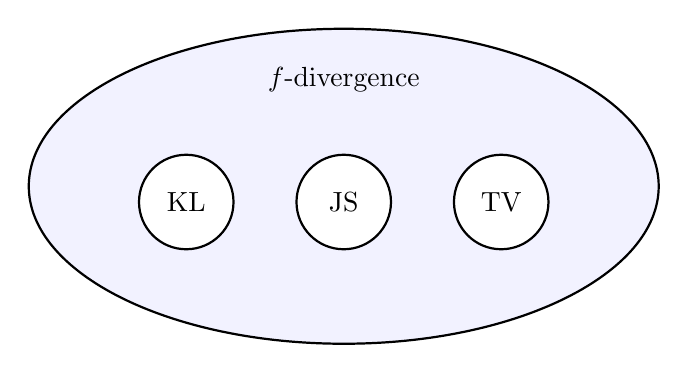
\begin{tikzpicture}
  \draw[thick, fill=blue!5] (0,0) ellipse (4cm and 2cm);
  \node at (0,1.35) {$f$-divergence};
  \node[draw, thick, circle, fill=white, minimum size=1.2cm] at (-2,-0.2) {KL};
  \node[draw, thick, circle, fill=white, minimum size=1.2cm] at (0,-0.2) {JS};
  \node[draw, thick, circle, fill=white, minimum size=1.2cm] at (2,-0.2) {TV};
\end{tikzpicture}


\end{frame}
%=======================================================
\begin{frame}{f-divergenceとKL-divergenceの関係}
    \begin{exampleblock}{forward KL}
        \centering$\mathit{f}(u)=u\log u \implies \mathcal{D}_{f}=\mathcal{D}_{KL}(p\mid\mid q)$\\
    \end{exampleblock}
    \begin{exampleblock}{}
    \centering$ \mathcal{D}_{f}(p\mid\mid q)=\int q(x)\mathit{f}\left(\frac{p(x)}{q(x)}\right)dx$\\
    \centering ここで$\mathit{f}(u)=u\log u$とすると、\\
    \begin{align*}
        \mathcal{D}_{f}(p\mid\mid q)
        &= \int q(x)\,f\Bigl(\frac{p(x)}{q(x)}\Bigr)\,dx \\
        &= \int q(x)\frac{p(x)}{q(x)}\log\frac{p(x)}{q(x)}\,dx \\
        &= \int p(x)\log\frac{p(x)}{q(x)}\,dx \\
        &= \mathcal{D}_{\mathrm{KL}}(p\mid\mid q)
    \end{align*}
    \end{exampleblock}
\end{frame}

%=======================================================
\begin{frame}{Jensen-Shannon divergence}
    \begin{exampleblock}{Jensen-Shannon}
        \centering$\mathit{f}(u)=\frac{1}{2}[u\log u-(1+u)\log\frac{(1+u)}{2}] \implies \mathcal{D}_{f}=\mathcal{D}_{JS}(p\mid\mid q)$\\
    \end{exampleblock}
        \begin{itemize}
        \item 対称性を持つ
        \item 非負性を持つ
        \item 一致時に0になる
    \end{itemize}
    $f(1)=0$は両分布が一致したときに評価値を0にするための条件\\
    凸関数であることは非負性を保証する\\
    $P(x)>0$ならば$m(x)>0$なのでKLのように比較先の密度が\\ゼロだから無限大になることはない


    \end{frame}
%=======================================================
\begin{frame}{f-divergenceとJensen-Shannon divergenceの関係}
    \begin{exampleblock}{}
    \small
    $\mathit{f}(u)=\dfrac{1}{2}\bigl[u\log u-(1+u)\log\dfrac{1+u}{2}\bigr]$
    とすると、
    \begin{align*}
    \mathcal{D}_{f}(p\mid\mid q)
    &= \int q(x)\,
       f\Bigl(\frac{p(x)}{q(x)}\Bigr)\,dx \\
    &= \frac{1}{2}\int
       \Bigl[
         p(x)\log\frac{p(x)}{q(x)}
         -(p(x)+q(x))\log\frac{p(x)+q(x)}{2q(x)}
       \Bigr]dx
    \end{align*}
    二つの分布の平均を
    $m(x)=\dfrac{p(x)+q(x)}{2}$
    とすると、
    \begin{align*}
        & p(x)\log\frac{p(x)}{q(x)}
          -(p(x)+q(x))\log\frac{m(x)}{q(x)} \\
        &= p(x)\Bigl[
             \log\frac{p(x)}{q(x)}
             -\log\frac{m(x)}{q(x)}
           \Bigr]
           -q(x)\log\frac{m(x)}{q(x)} \\
        &= p(x)\log\frac{p(x)}{m(x)}
           -q(x)\log\frac{m(x)}{q(x)}
        \end{align*}
        \centering$\therefore \mathcal{D}_{JS}(p\mid\mid q)=\frac{1}{2}\mathcal{D}_{KL}(p\mid\mid m)+\frac{1}{2}\mathcal{D}_{KL}(q\mid\mid m)$
    \end{exampleblock}
    \end{frame}
%=======================================================
\begin{frame}{total variation}
    \begin{exampleblock}{total variation}
        \centering$\mathit{f}(u)=\frac{1}{2}|u-1| \implies \mathcal{D}_{f}=\mathcal{D}_{TV}(p\mid\mid q)$\\
    \end{exampleblock}
    二つの分布の間で生じうる最大の確率の差を捉える尺度\footnote{別の見方として代表的な尺度ワッサーシュタイン距離(7章で扱う)}
    \begin{columns}[T]
        \begin{column}{0.48\textwidth}
            \begin{itemize}
                \item 対称性を持つ
                \item 非負性をもつ
            \end{itemize}
        \end{column}
        \begin{column}{0.48\textwidth}
            \begin{itemize}
                \item 一致時に0になる
                \item 三角不等式を満たす
            \end{itemize}
        \end{column}
    \end{columns}

    \begin{exampleblock}{}
    $\mathit{f}(u)=\frac{1}{2}|u-1|$とすると、
    \begin{align*}
        \mathcal{D}_{f}(p\mid\mid q)
        &=\frac{1}{2}\int q(x)|\frac{p(x)}{q(x)}-1|dx\\
        &=\frac{1}{2}\int q(x)|\frac{p(x)-q(x)}{q(x)}|dx\\
        &=\frac{1}{2}\int |p(x)-q(x)|dx\\
    \end{align*}
    \end{exampleblock}
\end{frame}
